\documentclass[twocolumn]{article}

\usepackage{graphicx}

%opening
\title{Tuning physic based solver}
\author{Rafael A. Fernandez Morera}

\begin{document}

\maketitle

\begin{abstract}
How similar a virtual product is to a real product is one of the most important issues when using virtual simulation to develop real apparel designs. The first step to achieve high similarity is finding optimal simulation parameters for the desired fabrics. However, it is notoriously difficult to find an optimal parameter set that reproduces the physical properties of a specific fabric as closely as possible. It is because the relationship between the changes of simulation parameters and drape shapes is highly non-linear, not intuitive, and hard to be predicted even by experts. Therefore, users have to repeat trial and error based on personal experience until they find satisfactory results, which is time consuming due to the simulation time required for each trial.

\end{abstract}

\section{Introduction}

To reproduce the drape characteristics of a real fabric through simulation, an appropriate set of simulation parameters for the fabric must be determined, which is the responsibility of the designer. Generally, simulation parameters represent the values of the physical and mechanical properties of the fabric. \cite{Ju2020}

One of the main problems with using the mechanical properties measured by the designer is that the physical mechanism of the cloth simulationis different from the mechanism of real cloth. Simulated drapes are often different from real drapes, even if you enter the precise mechanical properties \cite{Ju2020}.

One common ways for end users to ensure that their current set of simulation parameters is sufficient for the target fabric is to test the parameters on a simple drape such as the Cusick Drape Tester \cite{Ju2020} \cite{Cusick2008}.

If the real drape and the simulated drape are visually similar, the current set of simulation parameters can be considered adequate. However, if the drapes are different, the end user cannot be sure of the suitability of the simulation parameter set. In practice, designers iterate to adjust the simulation parameters until they get a simulated drape similar to the real drape, but tuning cloth simulation parameters is notoriously difficult. Even automatic optimization for a single target fabric takes at least a few hours.

In this study we present a method for obtaining representative textile simulation parameters from stable simulation of a differente solver, specifically NvFlex.

\section{Background}

In this paper, we extend the frontier in image understanding and present a method to recover the material properties of cloth from a video. We apply the Convolutional Neural Network (CNN) and the Long Short Term Memory (LSTM) neural network to material recovery of cloth from videos \cite{Yang2017}.

----

KES \cite{Kawabata2005} is the most representative instrument for measuring material. It precisely measures the mechanical properties of fabric, such as tensile strength, bending stiffness, and shear stiffness, as well as simple physical properties, such as frictional force and density. Most of these properties are the same as the simulation parameters used in general cloth simulators. Breen et al. \cite{Breen1994} directly used KES measurements as simulation parameters to simulate various cloth drapes, but they ignored the difference between the mechanism of the virtual simulator and the mechanism of real cloth. However, our goal is not to measure the actual mechanical properties of a real fabric but to estimate the simulation parameters that reproduce the desired static drape.

A. Hanging Drape Vs. Cusick’s Drape
The relationship between drapes and the mechanical properties of fabrics has been actively studied in the fields of textile engineering and computer graphics. In the field of computer graphics, the “hanging drape” has been most commonly used, in which a rectangular fabric specimen hung on a horizontal bar flutters due to artificial wind (see Fig. 1(a)). Most studies have estimated simulation parameters such as bending stiffness and weight from a video of the hanging drape for a specific fabric \cite{Bouman2013,Bhat2003,Davis2015,Yang2017,Bi}. The advantage of the hanging drape is that some physical properties, such as bending stiffness, are visually clear and can be perceived even with the naked eye. However, the downside is that it is difficult to recognize mechanical properties from a static image of a hanging drape [5], [8].

% TODO: \usepackage{graphicx} required
\begin{figure}
	\centering
	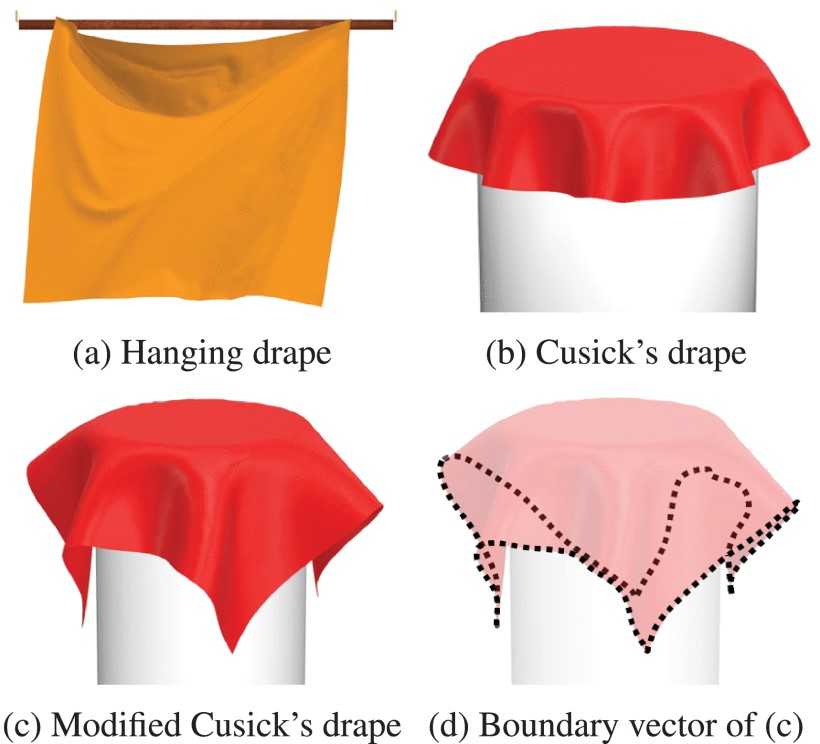
\includegraphics[width=0.7\linewidth]{choi1-3033765-large}
	\caption[Comparison of simulated hanging drape, Cusick’s drape, and our modified Cusick’s drape.]{}
	\label{fig:choi1-3033765-large}
\end{figure}

In the field of textile engineering, Cusick’s drape [1] or a variant thereof has been used to analyze various physical properties of fabrics. Cusick’s drape is formed by placing a circular fabric specimen over a small radius disk so that the edge of the specimen drops down (see Fig. 1(b)). Cusick’s drape is mainly observed after being projected as a 2D image onto a horizontal plane. For various analysis methods for Cusick’s drape, we refer to [9]. Numerous studies have demonstrated that Cusick’s drape is highly correlated with most KES measurements [10]–[13]. For example, Lam et al. [14] proposed a method for estimating the Cusick’s drape coefficient from mechanical properties of fabric using neural network learning. In addition, the Cusick’s method has evolved into a device for dynamic drape measurement and 3D drape shape analysis [15]–[18]. We also use the 3D geometric information of a variant of Cusick’s drape to estimate simulation parameters.

B. Optimizing Vs. Supervised Learning
Estimation of fabrics’ mechanical properties or simulation parameters has been studied through two major approaches. The first is an optimization approach, which iterates simulating and adjusting parameters until the desired drape is obtained. Bhat et al. [4] optimized simulation parameters to reproduce a desired hanging drape video. Wang et al. [19] and Miguel et al. [20] applied a certain force to fabric specimens using specially designed equipment to capture their deformations and then optimized the simulation parameters to reproduce the deformations. Mongus et al. [21] optimized the simulation parameters for the feature vector extracted from the Cusick’s drape of a target fabric. Yang et al. [22] optimized simulation parameters to reproduce the shape of the drape in a photo of a person wearing clothes. These optimization techniques have the advantage of not requiring training data. However, they require a long computation time. The methods mentioned above can take from several hours to tens of hours to optimize for a single fabric. Therefore, this approach is impractical for quickly simulating a variety of fabrics to find the most suitable one.

The second approach is to learn from training data. Most previous studies have used a series of hanging drape images as training data. Bouman et al. [5] and Bi et al. [8] used dozens of real fabric data to learn bending stiffness and weight from hanging drape images. Since their objective was to estimate the actual mechanical properties of fabric, they did not check whether the estimated values are valid for use as simulation parameters. Yang et al. [7] presented a learning method for estimation of simulation parameters. Hanging drape videos were created through simulation and used as training data. Rather than estimating the simulation parameter values directly, they simplified the problem into one that classifies 54 types of fabrics.

Our method is similar to [7] in that it learns from a set of training data generated through simulation. However, instead of a video of the hanging drape, we use a static drape inspired by Cusick’s drape, and we estimate simulation parameters directly rather than classify fabrics by type. Using a static drape makes it much easier to generate training data through simulation. In addition, forming a static drape of a specimen is more practical for end users compared to recording a video of cloth fluttering under a constant-intensity wind.

\bibliography{library}
\bibliographystyle{unsrt}
\end{document}
